\documentclass[18pt, a3paper, portrait]{tikzposter}
\usepackage[utf8]{inputenc}

\makeatletter
\def\title#1{\gdef\@title{\scalebox{\TP@titletextscale}{%
\begin{minipage}[t]{\linewidth}
\centering
#1
\par
\vspace{0.5em}
\end{minipage}%
}}}
\makeatother

\title{Machine Learning Techniques Used for Wind Turbine Monitoring}
\author{Yohann Jacob Sandvik}
\date{\today}
\institute{Institute of Electronic Systems - NTNU}
 
\usepackage{blindtext}
\usepackage{comment}
\usepackage{tikz} % To make cool diagrams
\usepackage{booktabs} % For fancy tables
\usepackage{tcolorbox} % To make colourful boxes (objectives)

\newcommand{\ra}[1]{\renewcommand{\arraystretch}{#1}} % Something about allowing more space between rows in fancy tables.
 
\usetheme{Envelope}
 
\begin{document}
 
\maketitle 

\begin{columns}
    \column{0.40}
    \block{The Wind Turbine}
    {
        \begin{tikzfigure}
            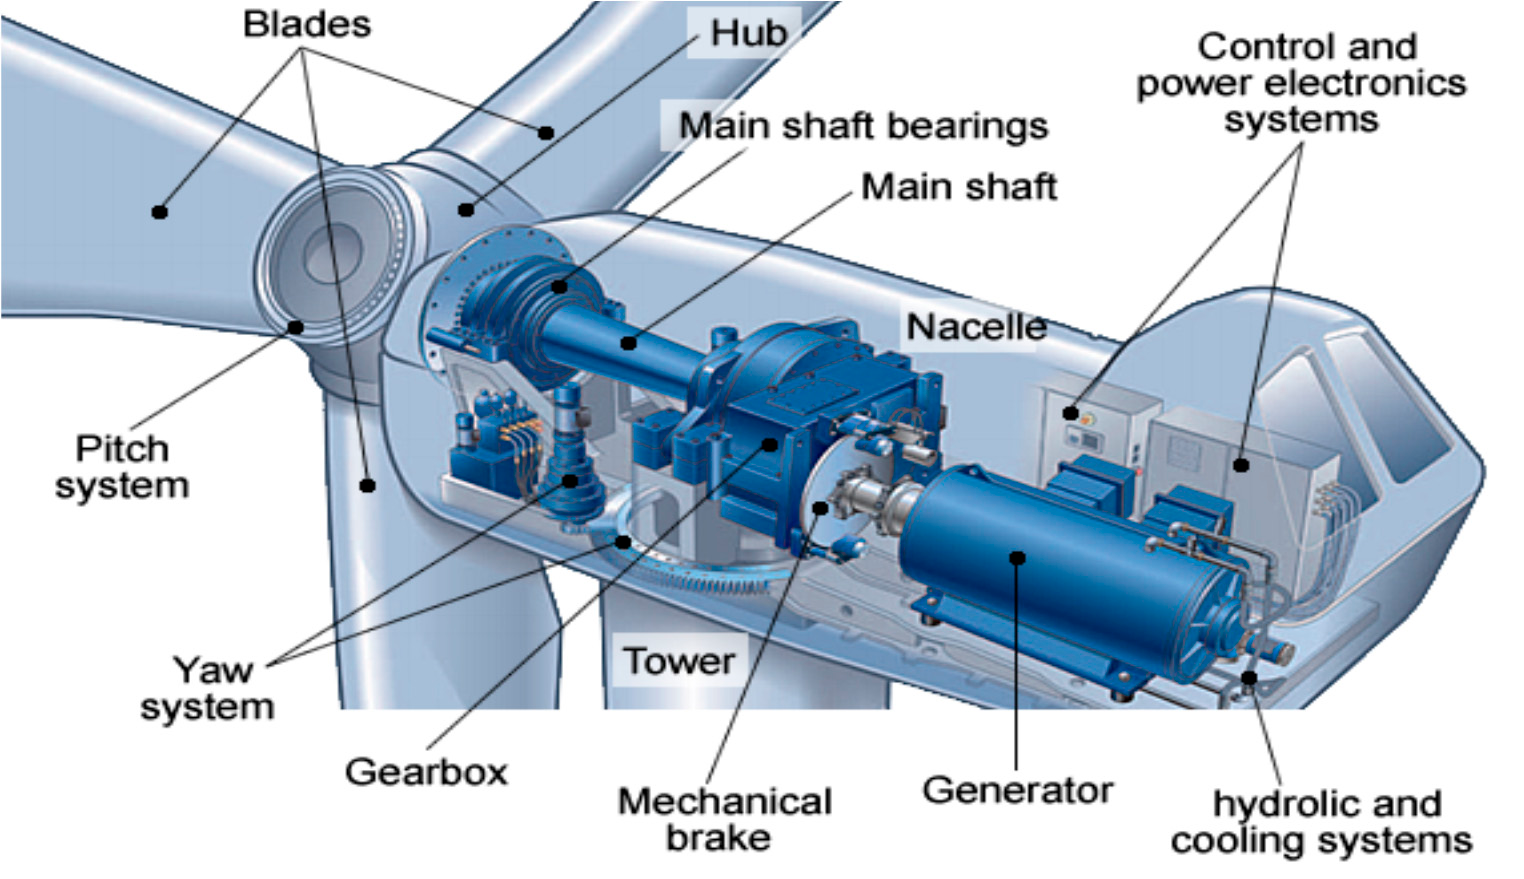
\includegraphics[width=0.35\textwidth]{images/wt_parts.png}
        \end{tikzfigure}
    }
 
    \column{0.60}
    \block{Objectives}
    {
        Simplified a wind turbine works by wind pushing the blades,
        generating torque that makes the hub rotate. The hub is connected to the gearbox through
        the main shaft. The gearbox then gears down the torque and gears up the rotational speed to
        a level that the generator can use to induce current, that goes to a station that transforms the
        voltage to a level that can be used in the electrical grid. \bigskip

        Information about a wind turbine can come from many sources, it can come from external
        sources such as images from a camera, or from internal sensors measuring operational data.
        The collective term for systems measuring operational data is supervisory control and data
        acquisition (SCADA) systems.
    }
\end{columns}

%% Regression based models 
\begin{columns}
    \column{0.40}
    \block{Table}
    {
        \begin{tikzfigure}
            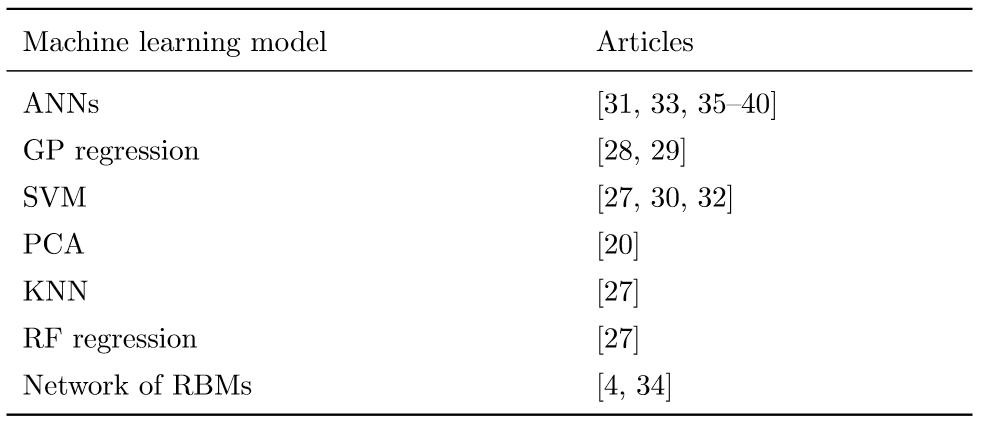
\includegraphics[width=0.35\textwidth]{images/regression_based_models_table.png}
        \end{tikzfigure}
    }
 
    \column{0.60}
    \block{Regression Based Models}
    {
        \begin{itemize}
            \item Abbreviations: Artificial Neural Networks (ANN), Support Vector Machine (SVM), Gaussian Process (GP), K-Nearest Neighbours (KNN), Principle Component Analysis (PCA), Random Forest (RF) and Restricted Boltzman Machine (RBM).
            \item A frequent approach is to use a supervised learning model to capture the normal behaviour
                of a wind turbine, or wind turbine component, by predicting the value of one time dependent
                variable, or by recreating the input variables.
            \item Then the deviation between the prediction and
                the actual value is used to detect anomalous behaviour.
            \item The authors then set a fixed threshold, or a variable threshold to which behaviour is considered anomolous.
        \end{itemize}
    }
\end{columns}

%% Supervised classification based models 
\begin{columns}
    \column{0.40}
    \block{Table}
    {
        \begin{tikzfigure}
            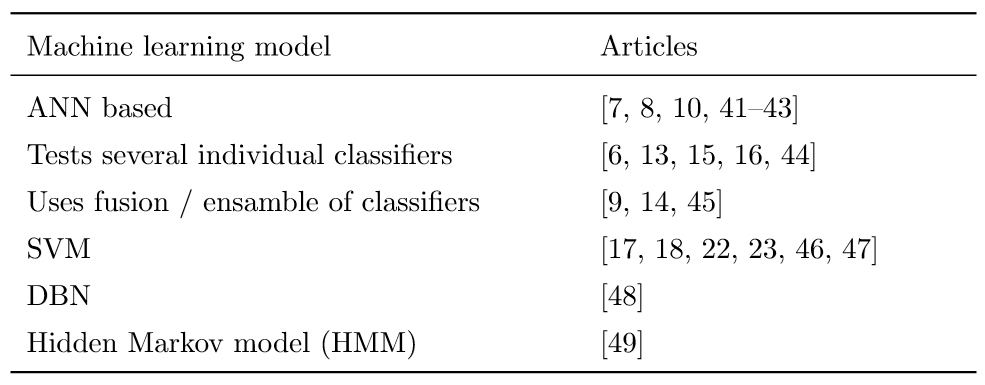
\includegraphics[width=0.35\textwidth]{images/supervised_clas_based_models_table.png}
        \end{tikzfigure}
    }
 
    \column{0.60}
    \block{Supervised Classification Based Models}
    {
        \begin{itemize}
            \item Abbreviations: Deep Belief Network (DBN).
            \item For supervised classifiers the models required labeled datasets to train. 
            \item Many of the supervised models use images to as input to detect damage in the blades.
            \item Many of the remaining models use vibrational sensors to detect structural damage in the blades as well.
        \end{itemize}
    }
\end{columns}

%% Unsupervised classification based models 
\begin{columns}
    \column{0.40}
    \block{Table}
    {
        \begin{tikzfigure}
            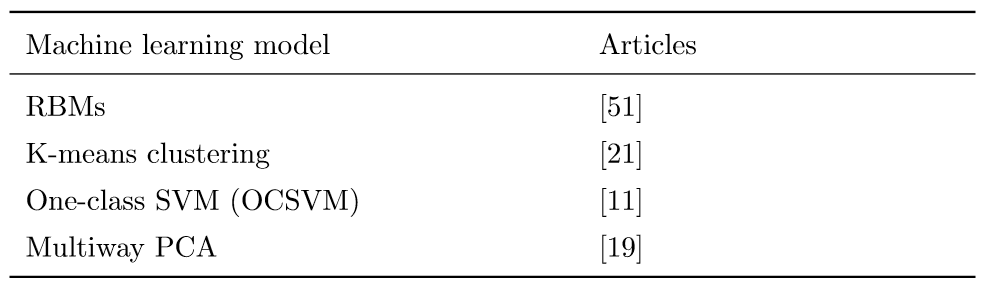
\includegraphics[width=0.35\textwidth]{images/unsupervised_clas_based_models_table.png}
        \end{tikzfigure}
    }
 
    \column{0.60}
    \block{Unsupervised Classification Based Models}
    {
        \begin{itemize}
            \item As evident from the tables, the unsupervised classification models are fairly rare compared to the supervised classification models. 
            \item There was found one implementation of clustering for condition monitoring of wind turbines, by Zhang and Ma [21]. 
                They use a generalization of PCA called parallell factor analysis (PARAFAC) for dimensionality reduction and K-means clustering on the reduced feature space.
                They are able to identify distinct operation modes of the wind turbines, and reduce data redundancy by PARAFAC. 
            \item However, they mention that there is still further work that can be done, especially in testing their model with data from turbines operating
                at different wind speeds.
            \item Pozo, Vidal, and Salgado [19] also have an interesting approach. They use multiway
                PCA to set up a baseline model, and then uses hypothesis testing to determine whether the
                power curve of a wind turbine is an anomaly or not.
        \end{itemize}
    }
\end{columns}

\block{Discussion}
{
    \begin{itemize}
        \item As can be expected to acheive high accuracy the amount of training data required, and the complexity of the model increases. Additionally, there is a trade-off between complexity and interpretability.
        \item The supervised classification based models are the most popular choice among the articles included, and show great promise in terms of accuracy, however they are quite hard to interpret. In addition, they require labelled datasets and the dataset available is not labelled so they are not considered relevant.
        \item The regression based models do not require explicit labeling to model normal behaviour, so they could be used to detect some anomalous behaviour. What is problematic with using complex regression based models is that without labelled data it might be hard to validate their performance.
        \item It is promising to see that K-means clustering paired with PARAFAC showed such good results.
    \end{itemize}
}
\end{document}


